\documentclass{article}
\usepackage{graphicx}
\usepackage{amsmath}
\usepackage[hyphens]{url}
\usepackage{hyperref}
\usepackage{float}

\begin{document}

\title{Graphics Pipeline}
\author{Justin Huffman, Eryn Kelsey-Adkins, Jesus Torres}

\maketitle

\begin{abstract}
The rendering pipeline is the series of steps a graphics system needs to follow to render a 3D scene to a 2D screen. These steps start with the Application, then the Geometry, the Rasterization, and finally the Display. This presentation provides a brief overview of each of the steps and the matrices used to transform 3D objects into 2D displays.
\end{abstract}

\section{Introduction}
3D graphics have become ubiquitous in the modern world. They are used in everything from movies to advertisements to, of course, computer games. Graphics applications like Blender and OpenGL make designing 3D graphics a relatively simply process, because they automate the transformations necessary to create and manipulate a 3D image and project it onto a 2D display.


The graphics pipeline is that series of steps needed to render a 3D scene to a 2D screen. \footnote{\url{https://commons.wikimedia.org/w/index.php?curid=58106609}}

\begin{figure}[H]
    \centering
    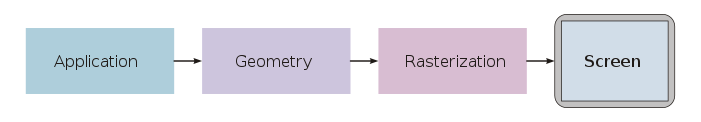
\includegraphics[width=3.0in]{Graphics_pipeline_2_en.png}
    \caption{By PaterMcFly / Vierge Marie}
    \label{pipeline}
\end{figure} 

This presentation provides a broad overview of these steps, focusing on the use of matrices in each transformation.

\section{Application: how 3D models are stored}

\subsection{World Coordinate System}
The world coordinates are the bedrock of the 3D model. This universal coordinate system is independent of the camera, and objects or primatives, which each have their own coordinate system, are placed within the world coordinates. Every point is defined by three vertices $(x, y, z)$. The cartesian coordinates can be left- or right- handed, defined by whether the z vertex points into or out of the display.\footnote{\url{cs.uic.edu}} Depending on the coordinate system being used, the models may need to be inverted when loading for veiwing.

\begin{figure}[H]
    \centering
    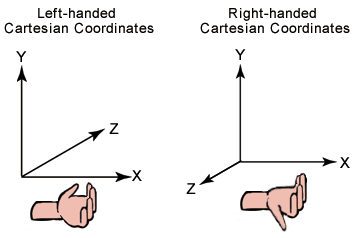
\includegraphics[width=3.0in]{leftrght.png}
    \caption{Left- and Right- Handed Cartesian Coordinates}
    \label{LeftRight}
\end{figure}

\subsection{Homogeneous Coordinates}
Instead of operating in $R^3$, most graphics pipelines use homogeneous coordinates, which exist in $R^4$ and are of the form $(x, y, z, w)$. Homogeneous Coordinates are useful because they allow the same transformations to be applied to both vertices (points in space that change when translated) and vectors (directions and facings, which do not).

A simple metaphor is to imagine a 2D projector. The X and Y values are easy to see, but what happens to the image as you move the projector closer or further away from the screen? The image is scaled up or down. This is similar to the w value in homogeneous coordinates.\footnote{\url{https://www.tomdalling.com/blog/modern-opengl/explaining-homogenous-coordinates-and-projective-geometry/}} 

For now we will set $w = 1$ for all vertices in our vertex list. If we had any vectors (i.e. normal vectors), we would set $w = 0$. (Other values of W will become relevent later in the projection step.) This will allow us to use the same standard $4x4$ matrices to tranform both vertices and vectors (should we need them for more advanced geometry calculations).

\subsection{Object Coordinate System}
As mentioned above, each object has its own set of coordinates. Objects are most often represented by polyhedren, further broken down into triangles. Each triangle is defined, possibly counterintuitively, by 4 vertices: the 3 edges, and a fourth vertex defining the front or face of the primative. When objects are moved in relation to the world coordinates, the origin of the object (in the object's coordinate system) is moved, with all other points transformed an equal amount.

Objects can further have a hierarchal coordinate system. The University of Illinois uses the example of a hand being positioned relative to the arm, rather than to the world coordinate system. 

\subsubsection{Polygon Mesh}
To build the Object Coordinate System, objects are represented by a polygon mesh: the vertices, edges, and faces that define the shape of the object. Faces consist of simple convex polygons to simplify rendering.\footnote{\url{https://commons.wikimedia.org/w/index.php?curid=10626667}}

\begin{figure}[H]
    \centering
    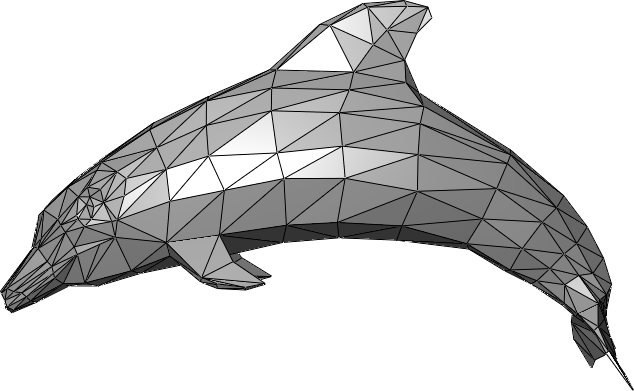
\includegraphics[width=3.0in]{Dolphin_triangle_mesh.png}
    \caption{An example of a Polygon Mesh}
    \label{dolphin}
\end{figure}

Vertices are connected to form edges, which are connected to form faces. Faces are connected into polygons; polygons are connected into surfaces, and finally, the surfaces are connected into the object.\footnote{\url{https://commons.wikimedia.org/w/index.php?curid=7021230}}

\begin{figure}[H]
    \centering
    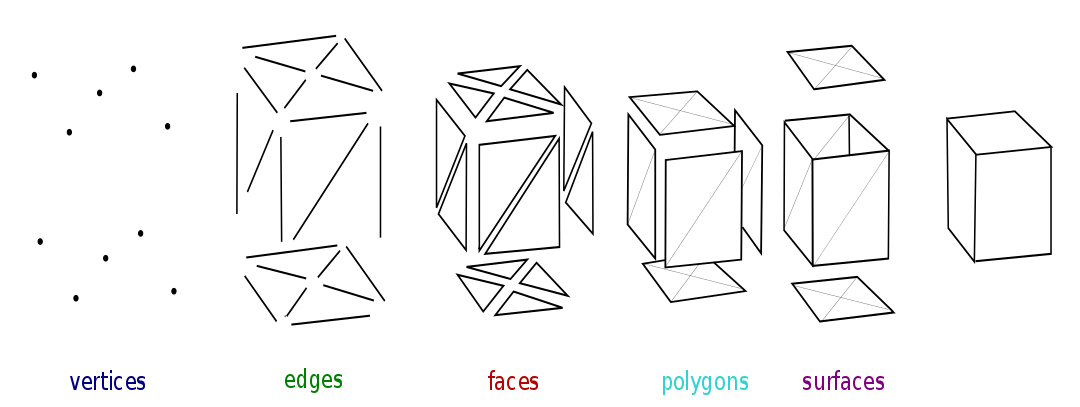
\includegraphics[width=3.0in]{Mesh_overview.png}
    \caption{Mesh Overview}
    \label{meshOverview}
\end{figure}

\subsubsection{Face-Vertex Mesh}
The most widely used mesh representation is the Face-vertex mesh. This representation is the input typically accepted by modern graphics hardware. The Face-Vertex Mesh stores model geometry in two parts. The first is a list of vertices. The second is a list of faces.\footnote{\url{https://en.wikipedia.org/wiki/Polygon_mesh\#Face-vertex_meshes}}

\begin{itemize}
\item{Vertex List:
List of vertices (points in 3D space), with each vertex being defined by its x, y, and z coordinates. Each vertex also contains a list of faces that it belongs to. (This is redundant, but saves having to search the face list for faces that a specific vertex belongs to.)}

\item{Face List:
A list of faces (most commonly triangles), with each face being defined by the three vertices that make it up. It is of the form (v1, v2, v3) where v1, v2, and v3 are references to points in the vertex list (usually the index of the vertex in the vertex array).

Since the connections between vertices do no change with normal geometric tranformations, most tranformations only deal with the vertex list with the face list not being used until the final clipping and rasterization steps.}
\end{itemize}

\subsection{Camera Transformation}
Once a world has been described with a World Coordinate System, and it has been populated by primatives, each with its own Object Coordination System, it is time to build the camera, or what the observer can see.

The camera transformation can be thought of as one more coordinate system: based upon the viewpoint of the observer, changing as the point of view changes. This coordinate system is defined  by:\footnote{\url{http://idav.ucdavis.edu/education/GraphicsNotes/Viewing-Transformation/Viewing-Transformation.html\#matrix}}

\begin{itemize}
\item A scene of the world coordinates, including all primatives within those coordinates
\item The camera position - $C = (x_{c}, y_{c}, z_{c})$
\item The point of the camera's focus - $A = (x_{a}, y_{a}, z_{a})$
\item The field of view angle - $\alpha$
\item The definition of the near and far planes, perpindicular to A with a distance of n and f from the camera
\end{itemize}

A pyramid is formed with C, A, and $\alpha$ which is then truncated by n and f into a frustum.

The transformation of the truncated viewing volume is given by:

\[A_{\alpha, n, f} = 
\begin{pmatrix}
\cot \frac{\alpha}{2} & 0 & 0 & 0 \\
0 & \cot \frac{\alpha}{2} & 0 & 0 \\
0 & 0 & \frac{f+n}{f-n} & -1 \\
0 & 0 & \frac{2fn}{f-n} & 0
\end{pmatrix}\]

\section{Geometry}

\subsection{Projection}
Projection transforms the view volume into a unit cube with extreme points at (1, 1, 1) and (-1, -1, -1). This step is called projection even though it is a volume to volume transformation because the z-coordinate is saved for the rasterization step.\footnote{Real-Time Rendering, Akenine-Möller, T., Haines, E., Hoffman, N.}

\subsubsection{Types of Projection}

\begin{figure}[H]
    \centering
    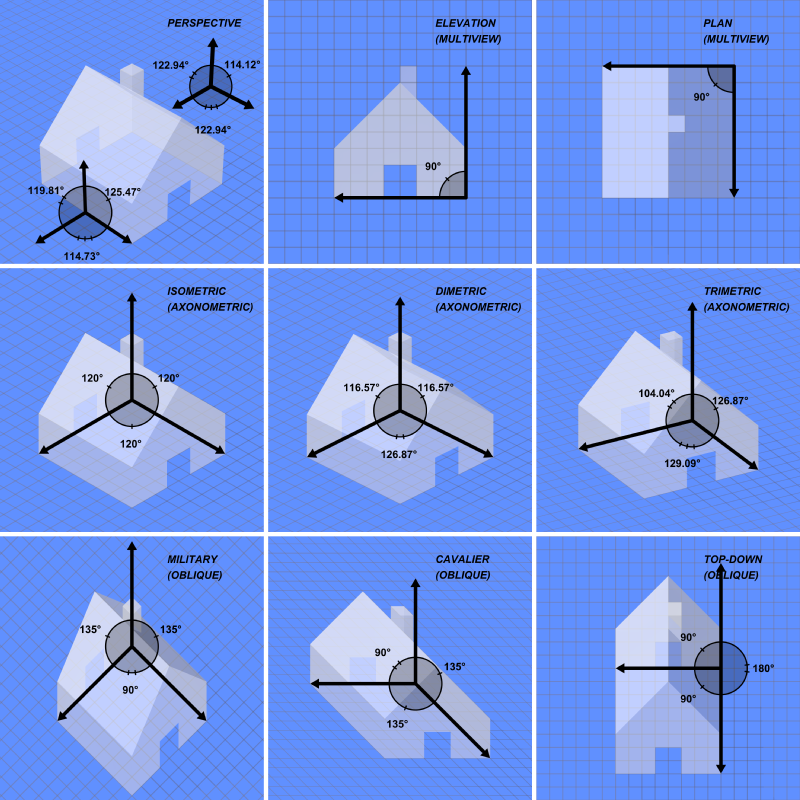
\includegraphics[width=3.0in]{Graphical_projection_comparison.png}
    \caption{A comparison of projection types}
    \label{projectiontypes}
\end{figure}

\subsubsection{Orthographic Projection}
Orthographic projection is mostly used in engineering for multi-view drawings. It is to scale, and all parallel lines remain parallel with no forced perspective. An orthographic projection transformation can be represented as:\footnote{Applied Geometry for Computer Graphics and CAD, Marsh, D.}

\[ P = \begin{pmatrix}
  1 & 0 & 0 & 0 \\
  0 & 1 & 1 & 1 \\
  0 & 0 & 0 & 0 \\
  0 & 0 & 0 & 1 
 \end{pmatrix}\]	


For each homogeneous vector $v = (v_x, v_y, v_z, 1)$, the transformed vector would be

\[P_{v} = \begin{pmatrix}
  1 & 0 & 0 & 0 \\
  0 & 1 & 1 & 1 \\
  0 & 0 & 0 & 0 \\
  0 & 0 & 0 & 1 
 \end{pmatrix}	
\begin{pmatrix}
  v_{x} \\
  v_{y} \\
  v_{z} \\
  1
 \end{pmatrix}	
=
\begin{pmatrix}
  v_{x} \\
  v_{y} \\
  0 \\
  1
 \end{pmatrix}\]

\subsubsection{Weak Perspective Projection}
Weak perspective projection adds a scaling factor to orthographic projection. This scaling factor uses averages to approximate perspective and is used with simple models and small fields of view.\footnote{Applied Geometry for Computer Graphics and CAD, Marsh, D.}

  \[P_{x} =  \frac{X}{Z_{ave}}\]
  \[P_{y} =  \frac{Y}{Z_{ave}}\]

assuming focal length $f = 1$.

\subsubsection{Perspective Projection}
Perspective projection most closely replicates the human binocular vision where distant objects appear smaller. To describe the transformation, we must start with four variables:\footnote{Applied Geometry for Computer Graphics and CAD, Marsh, D.}

\begin{itemize}
  \item $a_{x, y, z}$ - the 3D position of a point A that is to be projected
  \item $c_{x, y, z}$ - the 3D position of a point C representing the camera
  \item $\theta_{x, y, z}$ - the orientation of the camera
  \item $e_{x, y, z}$ - the display surface's positon relative to the camera pinhole. (Although negative z values are more correct, the create an inverted image both horizontally and vertically, so most conventions use positive values.
\end{itemize}

To compute the 2D projection ($b_{x, y}$) of the point A ($a_{x, y, z}$) that is to be projected, a vector $d_{x, y, z}$ is first defined as the position of point A with respect to the camera transformation, with origin in C and rotated by $\theta$:

\[\begin{pmatrix}
  d_{x} \\
  d_{y} \\
  d_{z} 
 \end{pmatrix}
=
\begin{pmatrix}
  1 & 0 & 0 \\
  0 & \cos(\theta_{x}) & \sin(\theta_{x}) \\
  0 &  -\sin(\theta_{x}) & \cos(\theta_{x}) 
 \end{pmatrix}
\begin{pmatrix}
  \cos(\theta_{y}) & 0 & -\sin(\theta_{y}) \\
  0 & 1 & 0 \\
  \sin(\theta_{y}) & 0  & \cos(\theta_{y}) 
 \end{pmatrix}\
\begin{pmatrix}
  \cos(\theta_{z}) & \sin(\theta_{z})  & 0  \\
  -\sin(\theta_{z}) & \cos(\theta_{z}) & 0 \\
  0 & 0  & 1 
 \end{pmatrix}\
\left(
\begin{bmatrix}
  a_{x} \\
  a_{y} \\
  a_{z} 
\end{bmatrix}\
-
\begin{bmatrix}
  c_{x} \\
  c_{y} \\
  c_{z} 
\end{bmatrix}\
\right)\]

\subsection{Clipping}
Clipping saves time and energy by specifying only those objects within the view volume for rendering. The vidual unit cube has been transformed into a truncated pyramid (frustrum) and objects outside of the frustrum are discarded by a method appropriately named frustrum culling. Objects that will be obscured by other primatives are also culled through backface culling. Objects inside the frustum are saved for rasterization.\footnote{\url{http://graphics.cs.cmu.edu/nsp/course/15-462/Spring04/slides/06-viewing.pdf}}

Objects that intersect the edges of the frustrum must be clipped. Line clipping simply modifies the endpoints of lines to lie within the appropriate rectangle. Polygon clipping converts a polygon that intersects the frustum into one or more polygons the form the intersection of the original with the clip window. The Sutherland-Hodgman Polygon Clipping Algorithm is commonly used\footnote{\url{https://www.geeksforgeeks.org/polygon-clipping-sutherland-hodgman-algorithm-please-change-bmp-images-jpeg-png/}}:

\begin{figure}[H]
    \centering
    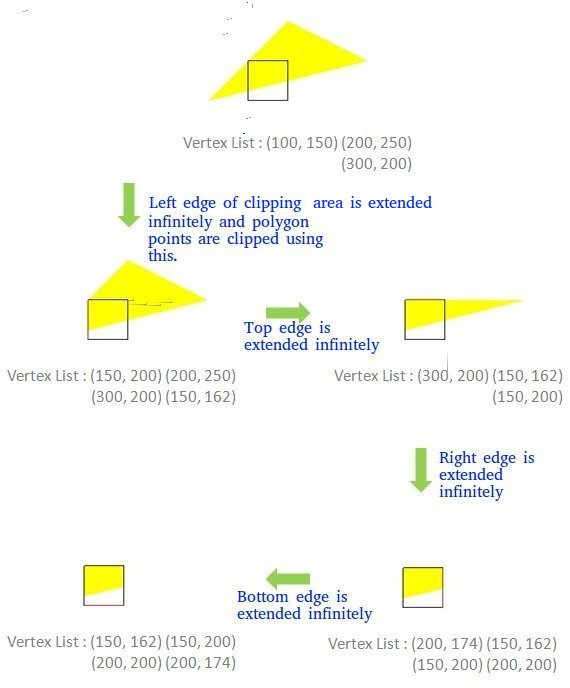
\includegraphics[width=3.0in]{Sutherland-Hodgman-Example.jpg}
    \caption{An example of the Sutherland-Hodgman Algorithm in use}
    \label{Sutherland-Hodgman}
\end{figure}

\subsection{Window-Viewport Transformation}
Translates camera coordinated into screen coordinated in order to match the size and location of the window

In order to be rendered on the screen, the camera coordinates need to first scaled and translated to match the coordinates of the target window (called the viewport).

\subsection{Rasterization}
Finally, the rasterization step computes the color that each pixel on the screen should be given the the relvent geomtry, lighting, and shaders.

Rasterization itself is a very complicated proccess, especially when taken into account things like lighting, textures, normal maps, and programmable shaders.

Here, we will limit ourselves to two of the most important steps: Z-buffering and line-drawing.

\subsubsection{Z-buffering}
A technique for detirmining which face is closest to the viewer, and therefore visable. Involves finding the z value of each polygon at each pixel, and then storing that value into the z-buffer and writing that polygon's RGB value to the frame buffer if it is lower than the z value already present in the buffer.

\subsubsection{Bresenham's line algorithm}
An algoritm for drawing a line using pixels between two points. Necessary for drawing a wireframe between the vertices of each face.

\section{Conclusion}
Write your conclusion here.

\end{document}
